%%% -*- TeX-master: "case-study.tex" -*-
\section{Discontinuous Galerkin Methods}
\label{sec:dg}

Discontinuous Galerkin methods (DG) are a class of numerical schemes for solving differential equations that draw on ideas from the finite volume as well as the finite element communities.
For simplicity's sake we will only consider one-dimensional problems.
Consider a spatial domain $X = [a, b] \subset \mathbb{R}$.
Let $u(x, t) : X \times \mathbb{R}_{\ge 0} \rightarrow \mathbb{R}$ be a scalar quantity defined on $X$ that varies with time $t$.
Furthermore consider the partial differential equation
\begin{equation}
  \label{eq:dg-pde}
  u_{t} + f(u)_{x} = 0
\end{equation}
that describes the behavior of $u$ where $u_{t}$ is $u$'s partial derivative with respect to time and $f(u)_{x}$ is the spatial derivative of some function $f$ of $u$.
Now given some boundary conditions, i.e. values for $u(a, t)$ and $u(b, t)$, and initial value conditions $u(x, 0)$ for all $x \in X, t \in \mathbb{R}_{\ge 0}$, we would like to solve equation \eqref{eq:dg-pde} for $u$.
The general approach which is also employed by DG is to
% TODO: Rewrite this
\begin{itemize}
\item discretize the domain spatially as well as timewise,
\item estimate the spatial derivatives from the known values at some point in time $t_{0}$,
\item solve \eqref{eq:dg-pde} for $u_{t}$
\item and finally use the derivatives with respect to time to approximate $u$ at a later point $t_{0} + \Delta t$.
\end{itemize}
So we will first discretize the spatial domain -- not necessarily uniformly -- into $n \in \mathbb{N}$ cells $[x_{i}, x_{i + 1}], i \in \{ 0, \dots, n - 1 \}$ such that the cells are ordered ($x_{0} < x_{1} < \dots < x_{n}$) and the resulting mesh covers the domain ($\cup_{i = 0}^{n - 1} [x_{i}, x_{i + 1}] = X$).

DG then approximates the solution $u$ from the data at each point in time $t$ by a piecewise continuous function $U$ that is continuous on the cell interiors but discontinuous at their boundaries.
These $U$ depend on $t$ but since the moment limiter does not work across timesteps we will now fix a time $t'$ for the rest of this section and all later mentions of $U$ will mean $U$ at time $t'$.
Written out we have
\begin{equation*}
  U = \bigoplus_{i = 0}^{n - 1} U_{i} \circ \xi_{i}
\end{equation*}
where $\oplus$ is a direct sum, $\circ$ is function composition, $U_{i}$ is a polynomial and $\xi_{i}$ normalizes coordinates in cell $i$ to the interval $[-1, 1]$, i.e. $\xi_{i}(x) = 2 \frac{x - x_{i}}{x_{i + 1} - x_{i}} - 1$.
The normalization is required because DG uses a special polynomial basis, the \emph{Legendre polynomials}.
So the $U_{i}$ can be written as
\begin{equation*}
  U_{i} = \sum_{j = 0}^{p} c_{i}^{j} P_{j}
\end{equation*}
where $P_{j}$ is the $j$-th Legendre polynomial and $U_{i}$ is of degree $p$.

There are two approaches to actually compute the polynomial approximations called \emph{nodal} and \emph{modal}.
Modal gives you polynomials in the form introduced here and is often preferred because the degree is easily adaptable; you just have to evaluate more or less coefficients.
Nodal on the other hand uses interpolation techniques to fit a polynomial which require data at specific points, called nodes, in a cell.
Since the nodes are completely different for each degree, this approach is not as amendable with regards to the polynomial degree and would require a complete recomputation for every change.
However, the moment limiter relies heavily on this operation, so going forward we will concentrate on modal DG.

How the solution $U$ is finally used to estimate the derivatives and advance the solution to the next timestep goes beyond the scope of this article.
The interested reader is encouraged to refer to \cite[chapter 3]{Hesthaven2007}.

Even though the model admits discontinuities at cell boundaries, it develops oscillations in their vicinity nonetheless as discontinuities and steep gradients pass through the cells.
This is demonstrated in figure \ref{fig:dg-oscillations} where a single shock was simulated for one complete traversal of a cyclic domain.
Such overshoots are not observed in physical processes and therefore stem entirely from numerical errors.

\begin{figure}[h]
  \centering
  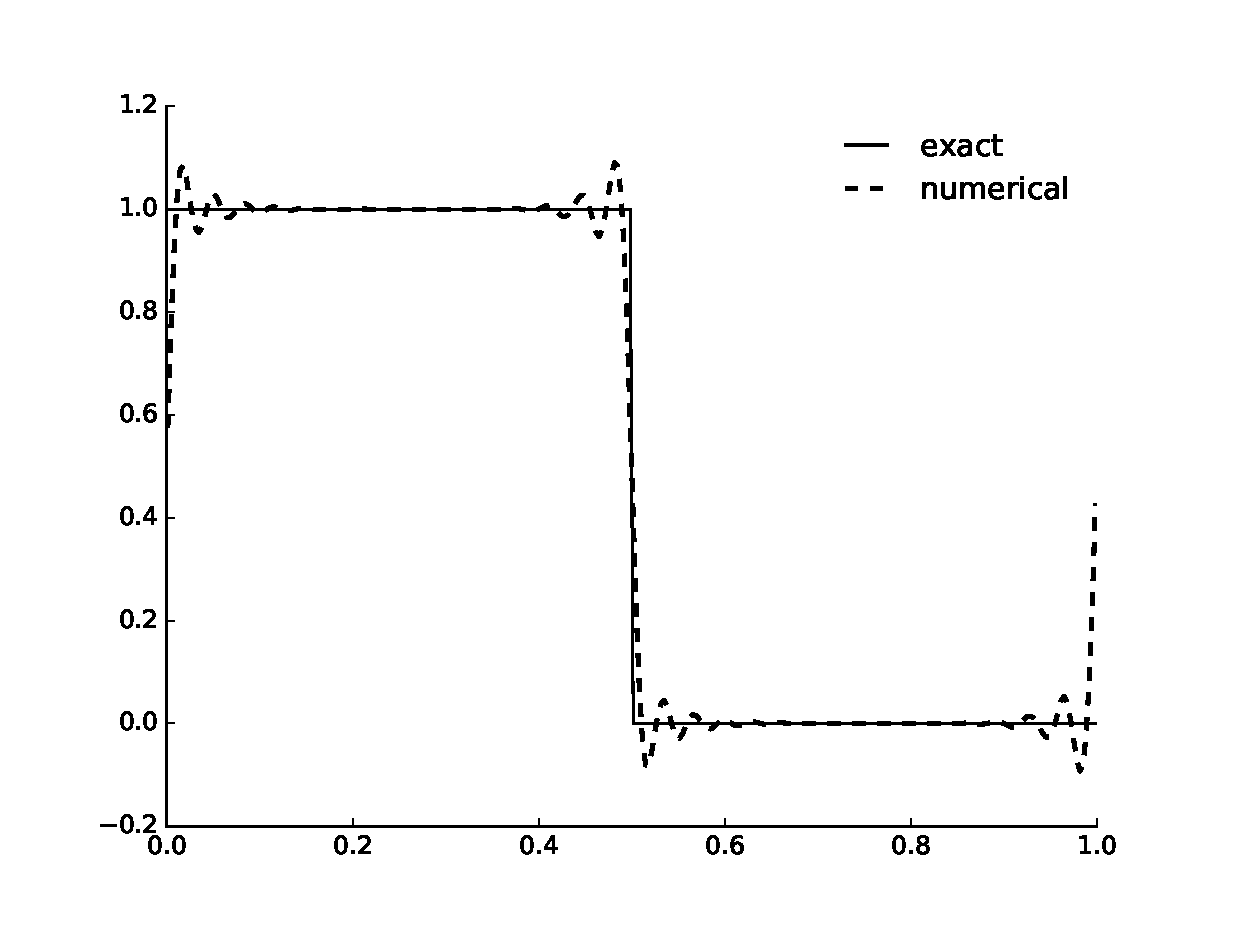
\includegraphics[width=0.8\columnwidth]{figures/oscillations}
  \caption{Linear advection of a shock; DG solution develops oscillations}
  \label{fig:dg-oscillations}
\end{figure}
